% Template authors: Bogumił Kamiński and Michał Jakubczyk
\documentclass[12pt,a4paper,twoside,openany]{book}
\usepackage[T1]{fontenc}
\usepackage[utf8]{inputenc}
\usepackage[polish]{babel}
\usepackage{csquotes}
\usepackage{graphicx}
\usepackage{times}
\usepackage{indentfirst}
\usepackage[left=3cm,right=2cm,top=2.5cm,bottom=2.5cm]{geometry}
\usepackage{enumitem}
\usepackage{color}
\usepackage{soul}
\usepackage{tikz}
\usepackage{url}
\usepackage{todonotes}
\usepackage{verbatim}

%\usepackage[square,authoryear]{natbib} % kluczowe
\usepackage[backend=biber,style=authoryear,sorting=nyt]{biblatex}
\addbibresource{bibliografia.bib}
\setlist{itemsep=0pt}
\setlist{nolistsep}
\frenchspacing
\linespread{1.3}
\addto\captionspolish{%
\renewcommand*\listtablename{Spis tabel}
\renewcommand*\tablename{Tabela}
}
\usepackage{titlesec}
\titlelabel{\thetitle.\quad}

\frenchspacing

\begin{document}

\begin{center}

\includegraphics[scale=0.3]{sgh_full.png}

\vspace{1cm}

% tu i dalej fbox należy usunąć i wpisać odpowiednią wartość
Studium magisterskie
\end{center}

\vspace{1cm}

\noindent Kierunek: Metody ilościowe w ekonomii i systemy informacyjne

\noindent Specjalność: Metody decyzyjne

\vspace{1cm}

{
\leftskip=10cm\noindent
Damian Płaskowicki\newline
Nr albumu: 117776

}

\vspace{2cm}

\title{Prototyp autonomicznego systemu handlującego na rynku forex wspieranego sztuczną inteligencją}
\makeatletter

\begin{center}
\LARGE\bf
\parbox{\textwidth}{\centering \@title}
\end{center}

\vspace{2cm}

{
\leftskip=10cm\noindent
Praca magisterska\newline 
napisana w Instytucie Finansów\newline
pod kierunkiem naukowym\newline
dr Ewy Cichowicz

}

\vfill

\begin{center}
Warszawa, \the\year
\end{center}

\thispagestyle{empty}

\clearpage
\thispagestyle{empty}
\mbox{}
% druga strona będzie pusta, ponieważ drukujemy dwustronnie
% a mbox jest po to, żeby ta strona się pokazała
% od procenta robimy komentarze
\clearpage

\tableofcontents

\clearpage

\chapter*{Wprowadzenie}

Współczesne rynki finansowe, w tym rynek walutowy Forex, charakteryzują się ogromną zmiennością, a do ich skutecznej analizy wykorzystuje się coraz większe ilości danych. W obliczu rosnącej złożoności analizy rynków inwestorzy instytucjonalni coraz częściej sięgają po zaawansowane narzędzia technologiczne, aby skuteczniej podejmować decyzje inwestycyjne. W ostatnich latach szczególną uwagę zyskały systemy wsparte sztuczną inteligencją (SI), które oferują nowe możliwości w zakresie analizy danych, prognozowania trendów rynkowych oraz automatyzacji procesu handlu. 

Celem tej pracy magisterskiej jest zaprojektowaie i wdrożenie w środowisku testowym prototypu w pełni autonomicznego systemu handlującego na rynku Forex, który w procesie podejmowania decyzji inwestycyjnych wykorzystuje metody sztucznej inteligencji. Prototyp ma na celu zademonstrowanie możliwości najnowszych technologi w autonomicznym handlu oraz sprawdzenie jego efektywności w warunkach rzeczywistych. W ramach pracy przeanalizowane zostaną różne podejścia do budowy autonomicznych systemów handlowych: oparte na sztucznej inteligencji, analizie technicznej oraz handlu wysokich częstotliwości.

Praca została podzielona na kilka etapów. Pierwszym krokiem jest zrozumienie podstawowych zasad funkcjonowania rynku Forex, jak również metod skutecznej spekulacji. Następnie przeprowadzona została analiza literatury, która pozwoliła wyodrębnić najbardziej obiecujące algorytmy oraz standardy rynkowe odnośnie projektowania tego typu systemów. Kolejnym etapem było projektowanie systemu, które obejmuje wybór odpowiednich algorytmów sztucznej inteligencji oraz architektury systemu. Następnie przeprowadzona została implementacja prototypu oraz testy wsteczne działania w symulowanych warunkach rynkowych. Na zakończenie, wyniki działania systemu zostaną poddane szczegółowej analizie, aby ocenić jego skuteczność, ograniczenia oraz możliwości dalszego rozwoju.

\chapter{Rynek walutowy}

\section{Historia i rozwój rynku walutowego}
\subsection{Starożytność}
Historia rynku walutowego sięga początków międzynarodowych stosunków gospodarczych. Jego rozwój był ściśle związany ze zmianami w systemach walutowych oraz rozwojem handlu międzynarodowego. 
Pierwsze formy wymiany walut powstały już w starożytności, kiedy wzrastał handel między europejskimi śródziemnomorskimi państwami oraz krajami bliskiego wschodu i azji. 
Wymianę barterową stopniowo zastępowała wymiana monetarna, w której o wartości monety decydowała zawartość kruszca, z której została ona wykonana. 
W rozwinętych włoskich miastach powstali pierwsi pośrednicy finansowi, zajmujący się wymianą walut o różnej zawartości kruszca i różnym pochodzeniu \parencite{melvin2013}. 

W kolejnych wiekach w starożytnym Rzymie powstał rozbudowany system monetarny oparty na srebrnym denarze, który stanowił podstawową jednostkę rozliczeniową w Imperium. 
Ujednolicenie wartości monet w oparciu o srebro umożliwiło rozwój handlu międzyregionalnego, co można uznać za wczesną formę zorganizowanego systemu walutowego \parencite{melvin2013}. 

\subsection{Średniowiecze}
Po upadku Cesarstwa Rzymskiegos ograniczono handel dalekosiężny, a znaczenie wymiany walutowej zmalało, lecz już w okresie średniowiecza powrócił w nowej formie. 
W europejskich miastach rozwijały się nowe prywatne instytucje finansowe zajmujące się wymianą walut, kredytem kupieckim oraz transferem środków między państwami. 
To właśnie w tym okresie powstały pierwsze weksle, listy kredytowe i rachunki rozliczeniowe, które można uznać za pierwowzory współczesnych instrumentów finansowych \parencite{mishkin2018}.

\subsection{XX wiek}
Przez większą część XX wieku funkcjonował system oparty na stałych kursach walutowych, którego podstawą był standard złota. 
Był systemem monetarnym, w którym wartość waluty krajowej opierała się na określonej ilości złota, a państwa utrzymywały stałe kursy wymiany między sobą. 
System ten zapewniał wysoką stabilność kursów walutowych, lecz ograniczał elastyczność polityki monetarnej, co ostatecznie doprowadziło do jego upadku w XX wieku \parencite{mishkin2018}.

Po II wojnie światowej przyjęto system z Bretton Woods, w ramach którego kursy walut powiązano z dolarem amerykańskim, a ten z kolei był wymienialny na złoto. 
System ten zapewniał względną stabilność międzynarodowych rozliczeń, jednak jego sztywność doprowadziła do narastających napięć gospodarczych \parencite{mishkin2018}. 

W 1971 roku prezydent Stanów Zjednoczonych Richard Nixon ogłosił zawieszenie wymienialności dolara na złoto, co w praktyce oznaczało koniec systemu z Bretton Woods. 
W kolejnych latach kraje zaczęły wprowadzać płynne kursy walutowe, co zapoczątkowało powstanie nowoczesnego rynku Forex w formie zdecentralizowanej sieci wymiany walut międzybankowych \parencite{hull2018}. 
Jak wskazuje Hull, upadek systemu stałych kursów był punktem zwrotnym w historii współczesnych finansów międzynarodowych, od tego momentu kursy walut zaczęły kształtować się w sposób rynkowy,
w oparciu o mechanizm popytu i podaży. 

Lata 80. i 90. XX wieku przyniosły gwałtowny rozwój rynku walutowego w związku z liberalizacją przepływów kapitałowych, rozwojem telekomunikacji oraz informatyzacji. 
W tym okresie pojawiły się pierwsze elektroniczne platformy transakcyjne, które zastąpiły tradycyjny rynek międzybankowy oparty na kontaktach telefonicznych. 
Z czasem rynek Forex zaczął przyciągać także inwestorów instytucjonalnych i detalicznych, co uczyniło go najbardziej płynnym rynkiem finansowym na świecie \parencite{zukowski2014}. 
Jak podaje Bank for International Settlements, dzienny obrót na globalnym rynku Forex wzrósł z około 590 miliardów dolarów amerykańskich w 1989 roku do ponad 7{,}5 biliona dolarów w 2022 roku \parencite{bis2022}.
Dane te obrazują skalę dynamicznego rozwoju tego rynku oraz jego rosnące znaczenie w światowym systemie finansowym. 

Na tle tych globalnych przemian również w Polsce zaczęły kształtować się warunki sprzyjające rozwojowi rynku walutowego. 
Początki rodzimego rynku Forex sięgają lat 90. XX wieku, kiedy to w wyniku otwarcia gospodarki i liberalizacji obrotu dewizowego możliwe stało się prowadzenie transakcji walutowych na szerszą skalę.
Początkowo uczestniczyły w nim głównie banki komercyjne, jednak wraz z postępem technologicznym i upowszechnieniem internetowych platform transakcyjnych rynek ten stał się dostępny również dla inwestorów indywidualnych.
Jak zauważają Furman i Hańczyk \parencite{furman2016}, istotną rolę w rozwoju krajowego segmentu rynku Forex odegrały zmiany regulacyjne oraz napływ zagranicznych brokerów internetowych.

Obecnie rynek Forex stanowi w pełni zdecentralizowany i globalny system wymiany walut, w którym uczestniczą zarówno banki centralne i komercyjne, jak i fundusze inwestycyjne, korporacje oraz inwestorzy detaliczni.
Jego ewolucja — od tradycyjnych kontaktów telefonicznych po nowoczesne platformy elektroniczne — odzwierciedla szersze procesy integracji rynków finansowych, cyfryzacji oraz globalizacji gospodarki światowej.

\section{Charakterystyka rynku Forex}

\subsection{Struktura i organizacja}

Rynek walutowy (Foreign Exchange Market, w skrócie Forex) jest rynkiem pozagiełdowym, co oznacza, że transakcje nie są zawierane na jednej scentralizowanej giełdzie,
lecz realizowane bezpośrednio pomiędzy uczestnikami za pośrednictwem sieci banków, brokerów oraz elektronicznych platform handlowych \parencite{bis2022}. 
Zdecentralizowany charakter rynku sprawia, że kursy walut kształtują się w sposób płynny w wyniku interakcji podaży i popytu w różnych centrach finansowych na całym świecie,
a nie w jednym punkcie notowań, jak ma to miejsce na tradycyjnych giełdach papierów wartościowych. 
Taka struktura sprzyja wysokiej elastyczności handlu, globalnemu zasięgowi oraz stałemu dostępowi do rynku niemal przez całą dobę.

Uczestnikami rynku Forex są różnorodne podmioty, które można podzielić na kilka głównych grup. 
Najważniejszą rolę odgrywają banki komercyjne i inwestycyjne, które stanowią głównych dostawców płynności, realizując transakcje zarówno między sobą, jak i ze swoimi klientami instytucjonalnymi. 
Istotnym uczestnikiem są również banki centralne, które wchodzą na rynek w celu stabilizacji kursów walutowych lub realizacji polityki monetarnej. 
Kolejną grupę stanowią korporacje międzynarodowe, dokonujące transakcji walutowych w związku z handlem zagranicznym, inwestycjami zagranicznymi czy zabezpieczaniem ryzyka kursowego. 
Ważną rolę pełnią także fundusze inwestycyjne oraz hedgingowe, które wykorzystują rynek do celów spekulacyjnych, arbitrażowych i zabezpieczających. 
W ostatnich latach coraz większe znaczenie zyskują również inwestorzy indywidualni, którzy dzięki rozwojowi technologii i internetowych platform tradingowych uzyskali bezpośredni dostęp do rynku \parencite{madura2018}. 
Motywacje uczestników rynku można zatem sprowadzić do trzech głównych kategorii: transakcyjnych, związanych z wymianą walut w działalności gospodarczej; 
zabezpieczających, czyli redukcji ryzyka kursowego; oraz spekulacyjnych, nastawionych na osiągnięcie zysku z krótkoterminowych zmian kursów.

Rynek Forex funkcjonuje nieprzerwanie przez 24 godziny na dobę, pięć dni w tygodniu. 
Handel rozpoczyna się w poniedziałek rano w Sydney, następnie przenosi się do Tokio, Londynu i Nowego Jorku, po czym cykl powtarza się aż do piątkowego wieczoru czasu nowojorskiego.
Dzięki temu uczestnicy rynku mają możliwość handlu w różnych strefach czasowych, co czyni Forex rynkiem o wyjątkowej ciągłości działania. 
Największa aktywność handlowa obserwowana jest w okresach nakładania się sesji europejskiej i amerykańskiej, kiedy płynność oraz zmienność są najwyższe \parencite{bis2022},
co ma miejsce zazwyczaj między godziną 13:00 a 17:00 czasu polskiego zimą (lub 14:00–18:00 latem), gdy jednocześnie aktywne są rynki w Londynie i Nowym Jorku.

Rynek Forex charakteryzuje się bardzo wysoką płynnością, co oznacza możliwość szybkiego zawierania transakcji o dużych wolumenach bez znaczącego wpływu na cenę rynkową. 
Według danych Banku Rozrachunków Międzynarodowych (BIS) z 2022 roku dzienny obrót na rynku walutowym przekraczał 7,5 biliona dolarów amerykańskich \parencite{bis2022}.
Tak ogromna skala obrotu sprawia, że Forex jest największym i najbardziej płynnym rynkiem finansowym na świecie.
Należy jednak zaznaczyć, że płynność nie jest stała w czasie. Zmienia się w zależności od pory dnia, aktywności poszczególnych centrów finansowych oraz publikacji istotnych danych makroekonomicznych,
które wpływają na zmienność kursów.

\subsection{Mechanizm działania rynku}

Transakcje na rynku Forex odbywają się zawsze w formie par walutowych, gdzie jedna waluta pełni funkcję waluty bazowej, a druga waluty kwotowanej. 
Kurs walutowy określa, ile jednostek waluty kwotowanej należy zapłacić za jedną jednostkę waluty bazowej. 
Przykładowo, kurs EUR/USD = 1,10 oznacza, że za jedno euro należy zapłacić 1,10 dolara amerykańskiego. 
Notowania walutowe są nieustannie aktualizowane w czasie rzeczywistym, a ich wartość kształtowana jest przez relację popytu i podaży na dane waluty na rynku globalnym \parencite{hull2018}. 
Najbardziej płynne i najczęściej handlowane pary walutowe określa się mianem „major pairs” i należą do nich: EUR/USD (euro do dolara amerykańskiego),
USD/JPY (dolar amerykański do jena japońskiego), GBP/USD (funt szterling do dolara amerykańskiego), USD/CHF (dolar amerykański do franka szwajcarskiego), 
AUD/USD (dolar australijski do dolara amerykańskiego) oraz USD/CAD (dolar amerykański do dolara kanadyjskiego). 
Pary te generują ponad 70\% całkowitego obrotu na rynku Forex, z czego wynika charakterystyczna dla nich wysoka płynność. 
Pary te charakteryzują się również dużym znaczeniem gospodarek emitujących dane waluty oraz szerokiej dostępności danych rynkowych \parencite{bis2022}. 
Pozostałe pary, określane mianem „minor pairs” lub „crosses”, obejmują waluty głównych gospodarek, ale bez udziału dolara amerykańskiego (np. EUR/GBP czy EUR/JPY), 
natomiast pary „egzotyczne” (\textit{exotic pairs}) łączą waluty gospodarek rozwiniętych z walutami krajów wschodzących, charakteryzując się niższą płynnością i wyższą zmiennością.

Transakcje walutowe mogą przybierać różne formy w zależności od horyzontu czasowego oraz celu ekonomicznego. 
Podstawowym rodzajem jest transakcja \textit{spot}, czyli natychmiastowa wymiana walut z rozliczeniem zazwyczaj w ciągu dwóch dni roboczych. 
Kolejnym typem są transakcje terminowe, do których należą kontrakty \textit{forward}, \textit{swap} oraz instrumenty pochodne, takie jak \textit{futures} i \textit{opcje walutowe}. 
Transakcje typu forward polegają na uzgodnieniu kursu wymiany w dniu zawarcia kontraktu, przy jednoczesnym ustaleniu przyszłego terminu jego realizacji, 
co pozwala uczestnikom zabezpieczyć się przed ryzykiem kursowym. Transakcje swapowe stanowią kombinację operacji kupna i sprzedaży tej samej waluty z różnymi datami rozliczenia, 
natomiast kontrakty futures i opcje walutowe są przedmiotem obrotu na rynkach regulowanych lub w ramach platform elektronicznych i służą zarówno do zabezpieczania pozycji, 
jak i do spekulacji \parencite{hull2018}.

Rynek Forex funkcjonuje w modelu dwustronnych kwotowań, w którym każdy instrument finansowy posiada dwa kursy: kurs kupna (\textit{bid}) i kurs sprzedaży (\textit{ask}). 
Różnica pomiędzy nimi, określana mianem \textit{spreadu}, stanowi podstawowy koszt transakcyjny oraz źródło zysku dla dostawców płynności, takich jak banki i brokerzy. 
Wysokość spreadu zależy od płynności danej pary walutowej, wolumenu transakcji oraz aktualnej zmienności rynkowej. 
Na najbardziej płynnych parach, takich jak EUR/USD czy USD/JPY, spread może wynosić zaledwie kilka jednostek pipsa, natomiast na parach egzotycznych jest zdecydowanie większy \parencite{bis2022}.

Istotną cechą handlu na rynku Forex jest wykorzystanie dźwigni finansowej (\textit{leverage}), która umożliwia inwestorom kontrolowanie pozycji o wartości wielokrotnie przewyższającej posiadany kapitał. 
Dźwignia pozwala na zwiększenie potencjalnych zysków, ale jednocześnie wiąże się ze znacznym ryzykiem poniesienia strat przekraczających depozyt zabezpieczający. 
Wysokość dostępnej dźwigni zależy od rodzaju uczestnika rynku, regulacji krajowych oraz polityki danego brokera. 
W przypadku inwestorów detalicznych w Unii Europejskiej, zgodnie z wytycznymi ESMA, maksymalna dźwignia dla głównych par walutowych wynosi 1:30, 
natomiast dla inwestorów profesjonalnych może być znacznie wyższa \parencite{esma2018}.

W praktyce handlu na rynku Forex istotną rolę odgrywa także wielkość jednostek transakcyjnych. 
Standardową jednostką obrotu jest tzw. \textit{lot}, odpowiadający 100 000 jednostkom waluty bazowej. 
Wraz z rozwojem rynku detalicznego wprowadzono mniejsze jednostki: \textit{mini lot} (10 000 jednostek) oraz \textit{mikro lot} (1 000 jednostek), które umożliwiły uczestnictwo inwestorom indywidualnym dysponującym mniejszym kapitałem \parencite{madura2018}. 
Handel przy użyciu mniejszych jednostek wiąże się jednak z relatywnie niższą wartością pozycji, przez co potencjalne zyski mogą być częściowo pochłonięte przez koszty transakcyjne.

W kontekście wykorzystania dźwigni finansowej szczególnie istotny jest wymóg utrzymywania tzw. depozytu zabezpieczającego (\textit{margin}), który stanowi część wartości otwartej pozycji. 
W przypadku niekorzystnych zmian kursu i spadku wartości depozytu poniżej wymaganego poziomu broker ma prawo do wezwania inwestora do jego uzupełnienia (\textit{margin call}) 
lub zamknięcia pozycji w celu ograniczenia dalszych strat. Oprócz spreadu inwestorzy ponoszą również inne koszty, takie jak prowizje od transakcji oraz tzw. \textit{swap}, 
czyli opłatę za utrzymanie otwartej pozycji przez noc. Swap odzwierciedla różnicę w stopach procentowych pomiędzy dwiema walutami tworzącymi parę i może mieć charakter dodatni lub ujemny, 
w zależności od kierunku transakcji i polityki monetarnej danego kraju \parencite{esma2018}.

Na kształtowanie kursów walutowych wpływa wiele czynników o charakterze zarówno ekonomicznym, jak i psychologicznym. 
Do najważniejszych należą różnice w poziomie stóp procentowych pomiędzy krajami, dane makroekonomiczne (takie jak inflacja, produkt krajowy brutto czy bilans handlowy), 
polityka monetarna banków centralnych oraz sytuacja geopolityczna. Dodatkowo, rosnący udział handlu algorytmicznego i automatyzacja procesów decyzyjnych sprawiają, 
że zmienność kursów może w krótkim okresie reagować na mikrostrukturalne czynniki rynkowe, takie jak wolumen obrotu czy publikacje danych w czasie rzeczywistym \parencite{chaboud2023}.

W przypadku inwestorów indywidualnych transakcje na rynku Forex realizowane są za pośrednictwem brokerów detalicznych, którzy udostępniają elektroniczne platformy transakcyjne, 
takie jak MetaTrader 4, MetaTrader 5 czy cTrader. Platformy te umożliwiają składanie zleceń kupna i sprzedaży w czasie rzeczywistym, monitorowanie notowań rynkowych, 
analizę techniczną oraz automatyzację handlu za pomocą tzw. ekspertów (EA – \textit{Expert Advisors}).

Inwestor może wybierać pomiędzy różnymi rodzajami zleceń, w tym zleceniami rynkowymi (\textit{market orders}), realizowanymi po bieżącej cenie rynkowej, oraz zleceniami oczekującymi (\textit{pending orders}), 
które aktywują się po osiągnięciu określonego poziomu ceny. Dodatkowo dostępne są mechanizmy zarządzania ryzykiem, takie jak zlecenia obronne \textit{stop loss} oraz zlecenia realizacji zysku \textit{take profit}, 
które automatycznie zamykają pozycję po osiągnięciu wyznaczonych progów.

Brokerzy mogą działać w różnych modelach rynkowych, m.in. \textit{Dealing Desk} (market maker), gdzie broker jest stroną transakcji i sam kształtuje kwotowania, 
lub w modelach \textit{STP} (Straight Through Processing) i \textit{ECN} (Electronic Communication Network), w których zlecenia klientów przekazywane są bezpośrednio na rynek międzybankowy. 
Model ECN charakteryzuje się zazwyczaj węższymi spreadami i większą transparentnością, lecz często wiąże się z dodatkowymi prowizjami transakcyjnymi.

Proces handlu u inwestorów detalicznych jest w pełni zautomatyzowany, a rozliczenia odbywają się w czasie rzeczywistym. 
Inwestor wpłaca środki w walucie bazowej rachunku (np. USD lub PLN), które stanowią depozyt zabezpieczający (\textit{margin}) i umożliwiają otwieranie pozycji z wykorzystaniem dźwigni finansowej. 
Całość procesu, od składania zleceń po rozliczenie, odbywa się elektronicznie bez fizycznej wymiany walut.

\subsection{Czynniki kształtujące kursy walutowe}

Kursy walutowe kształtują się w wyniku złożonych interakcji między wieloma czynnikami ekonomicznymi, politycznymi i rynkowymi. 
Jednym z najważniejszych czynników jest poziom stóp procentowych w poszczególnych krajach. 
Wyższe stopy procentowe przyciągają inwestorów zagranicznych, poszukujących wyższej stopy zwrotu, co prowadzi do zwiększonego popytu na walutę danego kraju i jej aprecjacji. 
Z kolei obniżki stóp procentowych często skutkują osłabieniem waluty, ponieważ zmniejszają atrakcyjność inwestycji denominowanych w tej walucie \parencite{madura2018}.

Istotne znaczenie mają również dane makroekonomiczne, takie jak tempo wzrostu gospodarczego (PKB), inflacja, poziom bezrobocia czy bilans handlowy. 
Pozytywne wyniki gospodarcze wzmacniają zaufanie inwestorów i przyczyniają się do wzrostu wartości waluty, natomiast słabe dane mogą prowadzić do jej deprecjacji. 
Na przykład wzrost inflacji powyżej oczekiwań rynkowych może sugerować konieczność zacieśnienia polityki monetarnej przez bank centralny, co często skutkuje umocnieniem waluty w krótkim okresie.

Znaczącym czynnikiem wpływającym na notowania walut są decyzje i komunikaty banków centralnych, które określają kierunek polityki pieniężnej. 
Oczekiwania dotyczące przyszłych zmian stóp procentowych, programów skupu aktywów (QE) czy interwencji walutowych mają natychmiastowy wpływ na rynki. 
Przykładowo, jastrzębie wypowiedzi przedstawicieli Rezerwy Federalnej (Fed) zazwyczaj prowadzą do umocnienia dolara amerykańskiego.

Nie bez znaczenia pozostają również czynniki geopolityczne i psychologiczne. 
Konflikty zbrojne, napięcia handlowe, kryzysy polityczne czy zmiany rządów mogą powodować gwałtowne przepływy kapitału w kierunku tzw. „bezpiecznych przystani”, 
takich jak dolar amerykański, frank szwajcarski czy złoto. 
Współcześnie dużą rolę odgrywają także czynniki behawioralne i nastroje inwestorów, które potrafią wzmacniać trendy rynkowe niezależnie od fundamentów ekonomicznych.

W ostatnich latach coraz większe znaczenie w kształtowaniu kursów walut zyskał handel algorytmiczny oraz automatyzacja procesów inwestycyjnych. 
Systemy oparte na sztucznej inteligencji i analizie danych w czasie rzeczywistym reagują błyskawicznie na publikacje makroekonomiczne i zmiany cen, 
co zwiększa krótkoterminową zmienność, zwłaszcza na najpłynniejszych parach walutowych \parencite{chaboud2023}.

\subsection{Statystyki i znaczenie rynku Forex}

Rynek walutowy pozostaje największym segmentem światowych finansów pod względem wartości obrotu. 
Według danych Banku Rozrachunków Międzynarodowych (BIS) z 2022 roku, dzienny obrót na globalnym rynku walutowym przekraczał 7,5 biliona dolarów amerykańskich,
z czego około 88\% wszystkich transakcji obejmowało dolara amerykańskiego \parencite{bis2022}. 
Oznacza to, że niemal każda operacja na rynku walutowym wiąże się z udziałem USD jako waluty bazowej lub kwotowanej, co czyni go bezsprzecznie najważniejszą walutą międzynarodową.
Na drugim miejscu znajduje się euro, które uczestniczy w 32\% transakcji, natomiast jen japoński w około 17\%. 
Udział pozostałych walut, w tym chińskiego juana (CNY) oraz funta szterlinga (GBP), systematycznie rośnie, co odzwierciedla przesuwanie się centrum ciężkości światowego handlu w kierunku Azji.

Na Rys.~\ref{fig:bis_turnover} przedstawiono średni dzienny obrót według rodzaju instrumentu. 
Widać wyraźnie, że największy udział mają transakcje typu \textit{FX swap}, które stanowią ponad połowę całkowitego obrotu, natomiast transakcje \textit{spot} odpowiadają za około jedną trzecią. 
Struktura ta jest typowa dla rynku międzybankowego, gdzie większość uczestników dokonuje transakcji o charakterze zabezpieczającym lub służących zarządzaniu płynnością, a nie spekulacji. 
Warto zauważyć, że mimo dominacji segmentu \textit{swap}, znaczenie transakcji natychmiastowych utrzymuje się na wysokim poziomie, 
co dowodzi stałego zapotrzebowania na bieżącą wymianę walut w globalnym handlu i finansach.

\begin{figure}[h!]
  \centering
  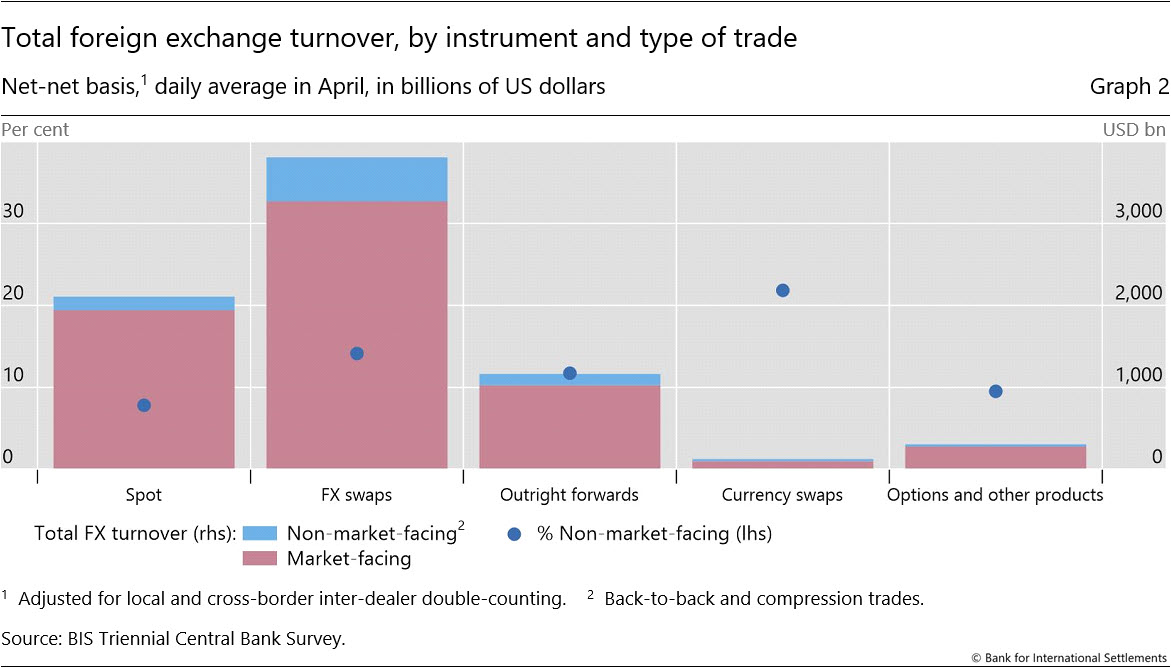
\includegraphics[width=0.85\textwidth]{plots/bis_fx_turnover_by_instrument_2022.jpg}
  \caption{Średni dzienny obrót na globalnym rynku walutowym według instrumentu w 2022 roku (w bln USD). Źródło: BIS (2022), \textit{Triennial Central Bank Survey}.}
  \label{fig:bis_turnover}
\end{figure}

Na poziomie walutowym (Rys.~\ref{fig:bis_pairs}) dominującą rolę odgrywa dolar amerykański (USD), który uczestniczy w 88\% wszystkich transakcji, 
a także euro (32\%) oraz jen japoński (17\%). Wśród najczęściej handlowanych par walutowych największy udział mają EUR/USD, USD/JPY oraz GBP/USD, 
co odzwierciedla dominację głównych gospodarek światowych w międzynarodowych przepływach kapitału. 
Warto zwrócić uwagę, że udział chińskiego juana (CNY) w obrotach Forex wzrósł w 2022 roku do około 7\%, co stanowi najwyższy poziom w historii i potwierdza rosnące znaczenie Chin w systemie finansowym. 
Mimo to udział walut rynków wschodzących wciąż pozostaje ograniczony z uwagi na niższą płynność i większe ryzyko regulacyjne.

\begin{figure}[h!]
  \centering
  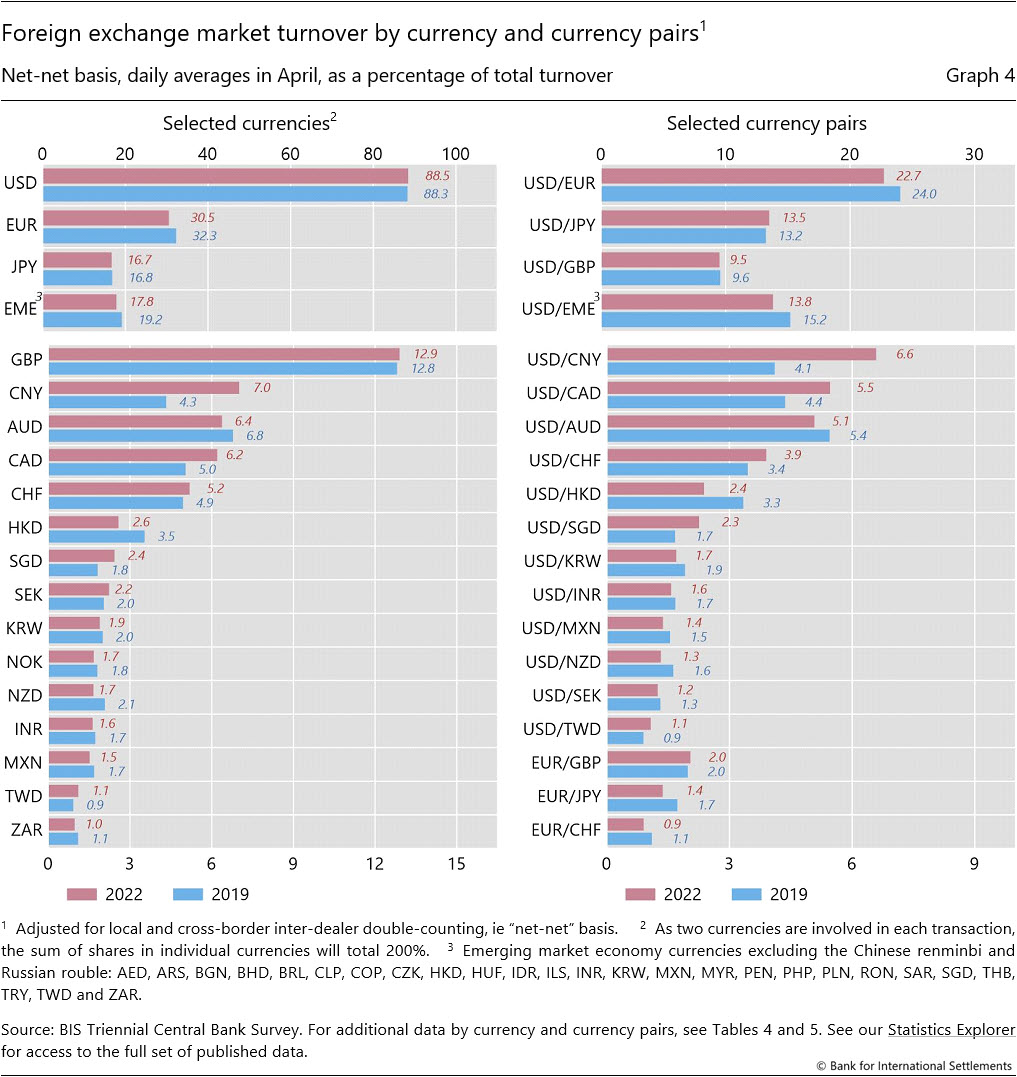
\includegraphics[width=0.9\textwidth]{plots/bis_fx_turnover_pairs_2022.jpg}
  \caption{Udział głównych walut i par walutowych w globalnym obrocie na rynku walutowym w 2022 roku (w \%). Źródło: BIS (2022), \textit{Triennial Central Bank Survey}.}
  \label{fig:bis_pairs}
\end{figure}

W kontekście Polski, zgodnie z wynikami badania Narodowego Banku Polskiego (NBP) z 2022 roku, średni dzienny obrót na krajowym rynku walutowym wyniósł około 13 miliardów dolarów amerykańskich,
co oznacza wzrost o ponad 47\% w porównaniu z 2019 rokiem \parencite{nbp2022}. Wzrost ten wpisuje się w globalny trend zwiększania aktywności na rynku walutowym po okresie pandemii COVID-19, 
który doprowadził do znacznych wahań kursowych i większej potrzeby zabezpieczania ekspozycji walutowych przez przedsiębiorstwa. 
Polska należy obecnie do grupy największych rynków walutowych w regionie Europy Środkowo-Wschodniej, wyprzedzając m.in. Czechy i Węgry. 
W strukturze obrotu dominują transakcje \textit{FX swap} (ok. 66\% obrotu) oraz \textit{spot} (ok. 24\%), co jest charakterystyczne dla rynków, 
na których dużą aktywność wykazują banki komercyjne i instytucje finansowe.

\begin{table}[h!]
\centering
\caption{Średni dzienny obrót na krajowym rynku walutowym według segmentów (kwiecień 2019 i 2022, w mln USD)}
\label{tab:nbp_segments}
\begin{tabular}{lccc}
\hline
Segment rynku & 2019 & 2022 & Zmiana (\%) \\
\hline
Transakcje spot & 2556 & 3130 & +22 \\
Forward & 959 & 1125 & +17 \\
FX swaps & 5190 & 8551 & +65 \\
CIRS & 41 & 87 & +112 \\
Opcje walutowe & 118 & 127 & +8 \\
\hline
\end{tabular}

\vspace{1mm}
{\footnotesize Źródło: opracowanie własne na podstawie NBP (2022).}
\end{table}

Analiza struktury walutowej krajowego rynku (Rys.~\ref{fig:nbp_breakdown}) pokazuje, że największy udział w obrocie mają pary z udziałem złotego polskiego, w szczególności EUR/PLN (ok. 51\%) i USD/PLN (ok. 22\%). 
Taka struktura wskazuje na silne powiązania gospodarki Polski ze strefą euro oraz znaczenie dolara jako waluty rozliczeniowej w handlu surowcami i inwestycjach międzynarodowych. 
Udział innych walut, takich jak funt brytyjski (GBP), frank szwajcarski (CHF) czy jen japoński (JPY), pozostaje relatywnie niewielki, co wynika z ograniczonego znaczenia wymiany handlowej z tymi krajami.
Warto przy tym zauważyć, że rosnący udział euro w obrocie na rynku krajowym jest także efektem intensywnej współpracy finansowej z bankami w krajach Unii Europejskiej.

\begin{figure}[h!]
  \centering
  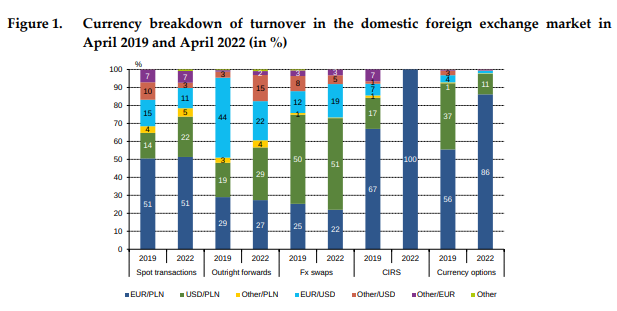
\includegraphics[width=0.85\textwidth]{plots/nbp_fx_poland_2022_breakdown.png}
  \caption{Struktura walutowa obrotu na krajowym rynku walutowym w Polsce w 2019 i 2022 roku (w \%). Źródło: NBP (2022), \textit{Wyniki badania rynku walutowego i rynku pozagiełdowych instrumentów pochodnych}.}
  \label{fig:nbp_breakdown}
\end{figure}

Z kolei struktura terminowa transakcji \textit{forward} i \textit{FX swap} wskazuje, że dominują operacje o krótkim horyzoncie – do siedmiu dni – które stanowią ponad 70\% wszystkich transakcji. 
Krótkoterminowy charakter obrotu potwierdza, że polski rynek walutowy służy przede wszystkim bieżącemu zarządzaniu płynnością i zabezpieczaniu pozycji, a nie długoterminowej spekulacji. 
Taka struktura jest typowa dla rynków rozwijających się, na których głównymi uczestnikami są banki komercyjne, instytucje finansowe i przedsiębiorstwa o ekspozycji na handel zagraniczny.

\begin{figure}[h!]
  \centering
  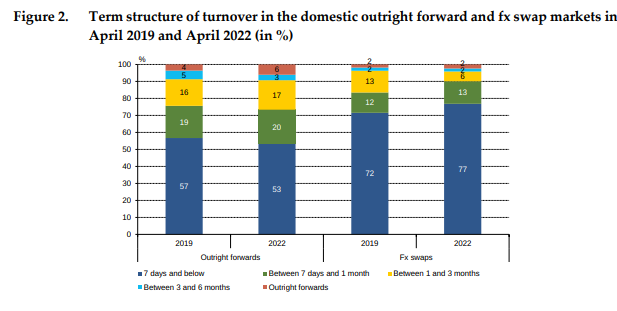
\includegraphics[width=0.8\textwidth]{plots/nbp_fx_poland_2022_swap.png}
  \caption{Struktura terminowa transakcji \textit{forward} i \textit{FX swap} na rynku krajowym w 2019 i 2022 roku (w \%). Źródło: NBP (2022).}
  \label{fig:nbp_swap_structure}
\end{figure}

Według danych Komisji Nadzoru Finansowego, w Polsce aktywnie inwestuje na rynku Forex około 80–100 tysięcy inwestorów detalicznych. 
Choć stanowią oni niewielki odsetek wszystkich uczestników rynku, ich rola stopniowo rośnie dzięki rozwojowi platform transakcyjnych i popularyzacji inwestowania online. 
Charakterystyczne jest jednak to, że większość obrotu generowana przez tę grupę ma charakter krótkoterminowy i spekulacyjny. 
Statystyki KNF wskazują, że około 70–80\% inwestorów detalicznych ponosi straty, co wynika przede wszystkim z wysokiego poziomu dźwigni finansowej oraz niedostatecznego zarządzania ryzykiem \parencite{knf2023}. 
Jednocześnie instytucje nadzorcze, w tym KNF i ESMA, prowadzą działania edukacyjne i regulacyjne, które mają na celu zwiększenie świadomości inwestorów i ograniczenie nadmiernego ryzyka w segmencie detalicznym.

Podsumowując, dane empiryczne BIS i NBP potwierdzają, że rynek walutowy, zarówno globalny, jak i krajowy, charakteryzuje się wysoką płynnością i dynamicznym wzrostem. 
W Polsce szczególnie istotną rolę odgrywają transakcje krótkoterminowe oraz operacje z udziałem złotego, które są ściśle związane z bieżącymi potrzebami finansowania handlu i zarządzania płynnością. 
Równocześnie rosnąca aktywność inwestorów indywidualnych, mimo wysokiego poziomu ryzyka, świadczy o zwiększającym się zainteresowaniu rynkiem Forex wśród uczestników detalicznych. 
Perspektywy dalszego rozwoju rynku w Polsce będą w dużej mierze zależeć od poziomu stabilności makroekonomicznej, 
regulacji europejskich oraz innowacji technologicznych wspierających dostęp do globalnych rynków finansowych.

\chapter{Spekulacja na rynku walutowym}

\section{Istota spekulacji}
Spekulacja odgrywa istotną rolę w funkcjonowaniu współczesnych rynków finansowych, w tym również rynku walutowego, wpływając na kształtowanie cen i płynność. 
W literaturze pojęcie to odnosi się do działań podejmowanych w celu osiągnięcia zysku z tytułu zmian cen aktywów finansowych, w szczególności w krótkim horyzoncie czasowym. 
Spekulanci nie są zainteresowani wartością fundamentalną instrumentu, lecz starają się przewidzieć kierunek jego przyszłych notowań.

Według klasycznej definicji przedstawionej przez Keynesa, spekulacja to „działanie mające na celu przewidywanie przyszłych zmian wartości aktywów, w przeciwieństwie do przedsiębiorczości, 
która polega na przewidywaniu przyszłej produktywności aktywów” \parencite{keynes1936}. 
Autor ten przestrzegał, że gdy spekulacja przejmuje kontrole nad rynkiem, wtedy staje się on niestabilny, tworząc tzw. "bańki spekulacyjne".
Współcześnie pojęcie spekulacji rozszerzono na wszelkie transakcje, których motywem jest zysk wynikający z oczekiwanych wahań cen rynkowych, niezależnie jakiego aktywa dotyczą \parencite{hull2018}. 
W ujęciu nowoczesnym spekulacja jest uznawana za proces inwestycyjny obarczony wysokim poziomem ryzyka, w którym zysk wynika z przewidywania krótkoterminowych zmian cen aktywów. 
Według Shleifera \parencite{shleifer2000}, spekulanci pełnią na rynku rolę podmiotów poszukujących okazji wynikających z nierównowagi cenowej, 
co w dłuższej perspektywie sprzyja zwiększeniu efektywności rynków finansowych.

Historycznie spekulacja była obecna na rynkach towarowych i kapitałowych na długo przed ukształtowaniem się współczesnego rynku walutowego. 
Kluczowym momentem dla rozwoju spekulacji walutowej był rozpad systemu z Bretton Woods i przejście do płynnych kursów, 
które w naturalny sposób zwiększyły zmienność i stworzyły przestrzeń dla strategii krótkoterminowych. 
Upowszechnienie elektronicznych platform, standaryzacja protokołów komunikacji międzydealerowej oraz niskie koszty transakcyjne doprowadziły do „demokratyzacji” dostępu, także dla inwestorów detalicznych \parencite{hull2018}.

Podstawowym celem spekulacji jest osiągnięcie zysku poprzez wykorzystanie krótkoterminowych wahań cenowych. 
W przeciwieństwie do inwestorów długoterminowych, którzy kierują się analizą fundamentalną i wartością wewnętrzną aktywów, spekulanci koncentrują się na analizie zachowań rynku oraz reakcji uczestników na napływ informacji \parencite{elder2014}. 
W kontekście rynku walutowego oznacza to dążenie do uzyskania zysku z różnic kursowych między parami walutowymi, 
przy czym horyzont czasowy transakcji może wynosić od kilku sekund (tzw. \emph{scalping}) do kilku dni lub tygodni (tzw. \emph{swing trading}) \parencite{murphy1999}. 
Warto zauważyć, że spekulacja różni się od klasycznego inwestowania również pod względem percepcji ryzyka i czasu ekspozycji na rynek. 
Inwestorzy zazwyczaj budują portfele zdywersyfikowane i utrzymują pozycje w dłuższym okresie, natomiast spekulanci koncentrują się na krótkoterminowych zmianach cen i wykorzystaniu dźwigni finansowej. 
Jak zauważa Hull \parencite{hull2018}, to właśnie wysoka zmienność oraz szybkie decyzje inwestycyjne odróżniają spekulację od tradycyjnych form lokowania kapitału.

Decyzje spekulantów rzadko są w pełni racjonalne. Badania z zakresu finansów behawioralnych pokazują wpływ heurystyk i błędów poznawczych, takich jak efekt stadny, 
nadmierna pewność siebie czy niechęć do ponoszenia strat \parencite{shleifer2000}. 
Krótkie horyzonty, wysoka dźwignia i częsta ekspozycja na informacje o wysokiej częstotliwości potęgują rolę emocji. 
Dlatego opracowanie reguł wejścia/wyjścia oraz limitowanie ryzyka jest tak samo ważna jak trafność prognozy.

Spekulacja jest często mylona z innymi strategiami finansowymi, takimi jak arbitraż i hedging, jednak różni się od nich zarówno celem, jak i profilem ryzyka. 
Arbitraż polega na wykorzystaniu różnic cenowych tego samego instrumentu finansowego na różnych rynkach lub w różnym czasie. 
Celem arbitrażu jest osiągnięcie zysku wolnego od ryzyka, co zasadniczo odróżnia go od spekulacji \parencite{fabozzi2015}. 
Z kolei hedging służy ograniczeniu ryzyka kursowego lub cenowego poprzez zawieranie transakcji zabezpieczających, które kompensują potencjalne straty z transakcji bazowych. 
W tym przypadku motywem działania nie jest zysk, lecz ochrona przed stratą \parencite{mishkin2019}. 
Spekulacja natomiast wiąże się z celowym przyjmowaniem ryzyka w nadziei na osiągnięcie ponadprzeciętnego zysku, co czyni ją bardziej ryzykowną, 
lecz jednocześnie niezbędną dla utrzymania równowagi i płynności rynku.

Rola spekulantów w systemie finansowym budzi liczne kontrowersje, jednak w ujęciu ekonomicznym ich działalność pełni istotną funkcję stabilizującą i informacyjną. 
Spekulanci zwiększają płynność rynku, ułatwiając zawieranie transakcji pomiędzy uczestnikami posiadającymi odmienne oczekiwania co do przyszłych kursów walut. 
Jak wskazuje Shleifer \parencite{shleifer2000}, ich działania przyczyniają się do efektywniejszego odkrywania cen oraz redukcji nieefektywności rynkowych wynikających z asymetrii informacji. 
Jednocześnie aktywność spekulantów może prowadzić do wzrostu krótkoterminowej zmienności kursów walutowych, szczególnie w okresach niestabilności makroekonomicznej lub politycznej. 
Mimo to większość badań empirycznych wskazuje, że obecność uczestników o charakterze spekulacyjnym przyczynia się do zwiększenia głębokości i płynności rynku, co z kolei poprawia jego funkcjonowanie \parencite{ mishkin2019}.

\section{Typy spekulantów}

Uczestnicy rynku walutowego różnią się między sobą pod względem motywacji, zasobów finansowych, dostępu do informacji oraz metod analizy rynku. 
W kontekście spekulacji walutowej można wyróżnić zarówno uczestników indywidualnych, jak i instytucjonalnych, przy czym obie grupy odgrywają istotną rolę w kształtowaniu płynności oraz dynamiki rynku \parencite{hull2018}. 
Różnorodność uczestników determinuje z kolei wykorzystywane strategie inwestycyjne oraz horyzonty czasowe spekulacji.

Spekulanci indywidualni, zwani również traderami detalicznymi, to osoby fizyczne prowadzące samodzielny handel na rynku Forex przy wykorzystaniu internetowych platform transakcyjnych. 
Zazwyczaj dysponują oni ograniczonym kapitałem oraz korzystają z wysokiej dźwigni finansowej, co umożliwia zajmowanie pozycji znacznie przekraczających ich rzeczywiste środki \parencite{elder2014}. 
Charakteryzuje ich krótki horyzont inwestycyjny oraz intensywne korzystanie z narzędzi analizy technicznej i automatycznych systemów transakcyjnych. 

Z kolei spekulanci instytucjonalni to profesjonalne podmioty dysponujące znacznymi zasobami finansowymi i technologicznymi. 
Wśród nich znajdują się banki inwestycyjne, fundusze hedgingowe, firmy tradingowe oraz wyspecjalizowane podmioty stosujące strategie wysokiej częstotliwości (HFT, ang. \emph{High-Frequency Trading}). 
Fundusze hedgingowe wykorzystują złożone strategie arbitrażowe, ilościowe oraz makroekonomiczne, a ich decyzje często wpływają na kierunek globalnych przepływów kapitałowych \parencite{fabozzi2015}. 
Z kolei algorytmy HFT, operujące w milisekundowych interwałach czasowych, generują ogromną liczbę zleceń w krótkim czasie, przyczyniając się do zwiększenia płynności, 
ale także do wzrostu krótkookresowej zmienności rynku \parencite{aldridge2013}.

\section{Strategie spekulacji}

Z punktu widzenia horyzontu czasowego wyróżnia się kilka podstawowych strategii spekulacji. Najkrótszym z nich jest \emph{scalping}, który polega na otwieraniu i zamykaniu pozycji w bardzo krótkich odstępach czasu, od kilku sekund do kilku minut. 
Celem tej strategii jest osiągnięcie wielu niewielkich zysków, wynikających z minimalnych wahań cenowych, przy jednoczesnym ograniczeniu ekspozycji na ryzyko rynkowe \parencite{murphy1999}. 

Kolejnym typem jest \emph{day trading}, w którym transakcje zawierane są w ciągu jednego dnia, bez przenoszenia pozycji na kolejną sesję. 
Taka strategia pozwala na uniknięcie ryzyka związanego z utrzymywaniem otwartych pozycji w nocy, gdy mogą wystąpić gwałtowne ruchy cen spowodowane wiadomościami spoza godzin aktywnego handlu.
Tego rodzaju strategia wymaga ciągłego monitorowania rynku i wysokiej dyscypliny inwestycyjnej.

Istotnym podejściem, często powiązanym z krótkoterminowymi strategiami, jest również \emph{news trading}.
Polega ono na podejmowaniu decyzji inwestycyjnych bezpośrednio w reakcji na publikacje danych makroekonomicznych, raportów korporacyjnych lub innych istotnych wiadomości rynkowych.
Strategia ta zakłada wykorzystanie chwilowej zwiększonej zmienności i płynności rynku, która pojawia się tuż po ogłoszeniu informacji.
Kluczowym elementem \emph{news tradingu} jest szybkość reakcji oraz dostęp do wiarygodnych źródeł danych, ponieważ nawet kilkusekundowe opóźnienie może zniwelować potencjalny zysk \parencite{harris2003}.

\emph{Swing trading} obejmuje horyzont średnioterminowy, zazwyczaj od kilku dni do kilku tygodni, i koncentruje się na wychwytywaniu krótkotrwałych trendów lub korekt w ramach większego ruchu cenowego. 
Strategia ta łączy elementy analizy technicznej i fundamentalnej, dzięki czemu pozwala na elastyczne dostosowanie decyzji inwestycyjnych do zmieniających się warunków rynkowych. 

Z kolei \emph{position trading} ma charakter długoterminowy i polega na zajmowaniu pozycji utrzymywanych przez wiele tygodni, a nawet miesięcy. 
W tym przypadku spekulanci opierają swoje decyzje przede wszystkim na analizie fundamentalnej, oczekując realizacji długoterminowych scenariuszy makroekonomicznych \parencite{hull2018}.

\section{Metody analizy rynku walutowego}

W literaturze przedmiotu strategie spekulacyjne na rynku walutowym klasyfikuje się zwykle według metod analizy, które stanowią ich podstawę. Pierwszą grupę stanowią strategie oparte na analizie fundamentalnej, w ramach których uczestnicy rynku prognozują zmiany kursów walut w oparciu o dane makroekonomiczne, takie jak poziom stóp procentowych, inflacja, bilans płatniczy, sytuacja budżetowa czy decyzje banków centralnych. Wśród technik stosowanych w analizie fundamentalnej wyróżnia się:
\begin{itemize}
    \item analizę parytetu siły nabywczej (PPP), określającą teoretyczny kurs równowagi wynikający z różnic poziomów cen;
    \item analizę parytetu stóp procentowych (IRP), badającą wpływ różnic w stopach procentowych na kursy terminowe;
    \item analizę bilansu płatniczego i rachunku obrotów bieżących, wskazującą kierunek przepływu kapitału między krajami;
    \item analizę decyzji banków centralnych oraz tzw. \emph{forward guidance}, czyli oczekiwań rynkowych dotyczących przyszłej polityki pieniężnej;
    \item modele długookresowej równowagi walutowej, takie jak FEER i BEER, stosowane do oceny fundamentalnej wartości walut \parencite{mishkin2019}.
\end{itemize}

Drugą grupę stanowią strategie oparte na analizie technicznej, w których decyzje inwestycyjne podejmowane są w oparciu o wykresy cenowe, wskaźniki techniczne i formacje trendów. Do najczęściej stosowanych technik należą:
\begin{itemize}
    \item analiza trendu za pomocą linii trendu i średnich kroczących (SMA, EMA, WMA), które służą do identyfikacji kierunku ruchu ceny;
    \item wykorzystanie wskaźników i oscylatorów, takich jak RSI (Relative Strength Index), MACD (Moving Average Convergence Divergence), Stochastic Oscillator oraz Bollinger Bands, które pozwalają ocenić siłę trendu, moment wykupienia lub wyprzedania rynku;
    \item analiza formacji cenowych (głowa i ramiona, podwójny szczyt, trójkąty, flagi) oraz świecowych (młot, doji, engulfing), umożliwiająca identyfikację punktów zwrotnych;
    \item analiza wolumenu transakcji i wskaźników typu OBV (On-Balance Volume), potwierdzająca siłę ruchu cenowego;
    \item analiza wielointerwałowa (multi-timeframe analysis), pozwalająca na określenie dominującego trendu w różnych skalach czasowych \parencite{elder2014}.
\end{itemize}

Trzecią, coraz bardziej dynamicznie rozwijającą się kategorię stanowią strategie algorytmiczne i ilościowe, które wykorzystują zaawansowane modele statystyczne, uczenie maszynowe oraz sztuczną inteligencję do automatycznego generowania sygnałów transakcyjnych. Wśród najczęściej stosowanych technik i metod można wymienić:
\begin{itemize}
    \item modele regresyjne (liniowe i nieliniowe) do przewidywania zmian kursów na podstawie historycznych danych cenowych;
    \item modele autoregresyjne i zmienności, takie jak ARIMA (Autoregressive Integrated Moving Average) i GARCH (Generalized Autoregressive Conditional Heteroskedasticity), służące do analizy dynamiki i ryzyka rynkowego;
    \item sieci neuronowe (MLP, LSTM) wykorzystywane do prognozowania kursów walut na podstawie sekwencji danych czasowych;
    \item algorytmy optymalizacji, takie jak algorytmy genetyczne, wykorzystywane do kalibracji parametrów modeli handlowych;
    \item strategie oparte na analizie sentymentu rynkowego i przetwarzaniu języka naturalnego (NLP), analizujące komunikaty agencji informacyjnych, media społecznościowe i wypowiedzi banków centralnych;
    \item systemy HFT wykorzystujące arbitraż statystyczny i mikrosygnały rynkowe do otwierania i zamykania pozycji w ułamkach sekund \parencite{hull2018}.
\end{itemize}

Wybór metody analizy rynku walutowego również odzwierciedla motywacje i cechy inwestora. 
Inwestorzy nastawieni na szybki zysk wybierają metody o wysokiej reaktywności, takie jak analiza techniczna i wskaźniki krótkoterminowe. 
Inwestorzy o motywacji poznawczej lub instytucjonalnej preferują modele ilościowe i algorytmy statystyczne, natomiast uczestnicy o motywacjach defensywnych, 
wybiorą analizę fundamentalną i długoterminowe prognozy makroekonomiczne. 
Takie zróżnicowanie metod wskazuje, że spekulacja na rynku walutowym nie jest jednolitym procesem, lecz wielowymiarowym zjawiskiem łączącym ekonomię, psychologię i technologię.

Współczesne podejście do spekulacji coraz częściej łączy elementy analizy fundamentalnej, technicznej i ilościowej, 
tworząc hybrydowe strategie handlu, które są w stanie adaptować się do zmiennych warunków rynkowych. 
Takie rozwiązania wspierane są przez sztuczną inteligencję i uczenie maszynowe, co pozwala na automatyczne dostosowanie parametrów strategii w odpowiedzi na zmiany zmienności, 
płynności oraz struktury rynku. 
Hybrydowe podejście stanowi fundament rozwoju autonomicznych systemów handlu walutowego, które stanowią przedmiot dalszych rozważań w kolejnych rozdziałach niniejszej pracy.

Spekulacja na rynku walutowym stanowi złożony proces, w którym zyski i straty wynikają nie tylko z analizy ekonomicznej, ale również z indywidualnych motywacji, emocji i zdolności adaptacyjnych inwestorów. 
Dopasowanie strategii do profilu psychologicznego i motywów działania zwiększa szansę na osiągnięcie sukcesu, minimalizując jednocześnie wpływ błędów poznawczych. 
Współczesny rynek walutowy, charakteryzujący się wysoką zmiennością i niskimi barierami wejścia, wymaga od uczestników nie tylko wiedzy technicznej, ale również samoświadomości i dyscypliny inwestycyjnej. 
Zrozumienie relacji między motywacją a strategią stanowi zatem fundament skutecznego uczestnictwa w procesie spekulacyjnym.

\section{Psychologiczne aspekty spekulacji i zarządzanie emocjami}

Spekulacja na rynku walutowym wiąże się z silnym komponentem psychologicznym, ponieważ decyzje inwestycyjne podejmowane są często w warunkach niepewności, presji czasowej i emocjonalnego napięcia. 
Jak zauważa Kahneman \parencite{kahneman2011}, ludzki umysł działa w dwóch trybach: szybkim, intuicyjnym (System 1) oraz wolnym, analitycznym (System 2). 
W kontekście spekulacji walutowej oznacza to, że traderzy często podejmują decyzje impulsywnie, reagując na bieżące wahania rynku, zamiast kierować się racjonalną analizą danych. 

Najczęściej występującymi błędami poznawczymi wśród spekulantów są: nadmierna pewność siebie, efekt potwierdzenia (tendencja do poszukiwania informacji zgodnych z własnymi przekonaniami), 
awersja do strat oraz efekt świeżości, polegający na przecenianiu ostatnich wydarzeń kosztem długoterminowych trendów \parencite{shefrin2007}. 
Takie zachowania prowadzą do nadmiernego handlu, zbyt wczesnego zamykania zyskownych pozycji lub odwlekania realizacji strat. 

Według Eldera \parencite{elder2014}, skuteczny trader powinien wypracować wysoki poziom dyscypliny emocjonalnej i konsekwentnie przestrzegać przyjętych zasad zarządzania ryzykiem. 
Pomocne jest prowadzenie tzw. dziennika transakcyjnego, w którym zapisywane są motywacje i emocje towarzyszące każdemu zleceniu. 
Dzięki temu inwestor uczy się rozpoznawać wzorce zachowań i ograniczać wpływ emocji na decyzje finansowe. 

W literaturze wskazuje się, że utrzymanie obiektywnego podejścia do rynku wymaga stosowania tzw. procedur automatyzujących decyzje, takich jak zlecenia stop-loss, 
limity strat dziennych czy określenie maksymalnej liczby transakcji w ciągu sesji. 
Mechanizmy te redukują wpływ emocji i zwiększają szansę na zachowanie spójności strategii. 
Jak podkreśla Shefrin \parencite{shefrin2007}, w długim okresie to nie trafność prognoz, lecz zdolność kontroli emocji decyduje o sukcesie na rynku spekulacyjnym.

\section{Motywy podejmowania spekulacji}

W praktyce decyzje o podjęciu działalności spekulacyjnej wynikają z różnych motywów inwestorów. 
Dla części z nich jest to chęć osiągania ponadprzeciętnych zysków w krótkim czasie, dla innych, potrzeba emocji, samorealizacji lub przynależności do społeczności inwestycyjnej.  
W literaturze przedmiotu \parencite{shefrin2007} wyróżnia się trzy główne grupy motywów:

\begin{itemize}
\item \textbf{Motyw zysku ekonomicznego} - dominujący wśród inwestorów instytucjonalnych, którzy dążą do maksymalizacji stopy zwrotu przy akceptowalnym poziomie ryzyka. 
Ich działania są najczęściej oparte na modelach ilościowych i analizie danych.
\item \textbf{Motyw emocjonalny i prestiżowy} - typowy dla inwestorów indywidualnych, dla których spekulacja stanowi formę rywalizacji, 
źródło satysfakcji lub sposób na potwierdzenie własnych kompetencji finansowych.
\item \textbf{Motyw informacyjny} - charakterystyczny dla uczestników rynku poszukujących przewagi wynikającej z dostępu do informacji, 
analizy danych lub technologii (np. algorytmy HFT, modele predykcyjne AI).
\end{itemize}

Jak zauważa Barberis i Thaler \parencite{barberis2003}, motywacje te wpływają na sposób postrzegania ryzyka oraz na wybór strategii, 
co w konsekwencji prowadzi do zróżnicowania zachowań spekulacyjnych na rynku walutowym.

Wybór strategii spekulacyjnej powinien być zgodny z motywami i cechami psychologicznymi inwestora. W literaturze wyróżnia się kilka typów profili inwestycyjnych, które determinują styl podejmowania decyzji na rynku walutowym \parencite{shefrin2007}:

\begin{itemize}
\item \textbf{Inwestor agresywny} - kieruje się motywem osiągnięcia wysokiego zysku w krótkim czasie. 
Charakteryzuje go wysoka tolerancja na ryzyko, impulsywność i skłonność do używania dźwigni finansowej. 
Typowymi strategiami wykorzystywanymi przez tego typu inwestowa są \emph{scalping}, \emph{day trading} oraz handel na danych makroekonomicznych (tzw. \emph{news trading}).
\item \textbf{Inwestor zrównoważony} - poszukuje równowagi między zyskiem a bezpieczeństwem kapitału. 
Skłonny do analizy technicznej i fundamentalnej w średnim horyzoncie (\emph{swing trading}), preferuje umiarkowaną dźwignię i ograniczone ryzyko transakcyjne.
\item \textbf{Inwestor defensywny} - unika nadmiernej zmienności, często wykorzystuje analizy fundamentalne i makroekonomiczne. Wybiera strategie oparte na długoterminowych trendach (\emph{position trading}),
stosuje niską dźwignię i dużą dywersyfikację.
\end{itemize}

Dodatkowo, coraz częściej analizuje się rolę \textbf{motywacji poznawczych}, takich jak chęć uczenia się, testowania hipotez rynkowych czy budowania modeli ilościowych. 
Takie postawy są charakterystyczne dla inwestorów akademickich, analityków danych oraz firm tradingowych, które opierają się na strategiach algorytmicznych.

Związek między motywacją a strategią można przedstawić w tabeli:

\begin{table}[h!]
\centering
\caption{Dopasowanie strategii do profilu inwestora}
\begin{tabular}{lll}
\hline
Profil inwestora & Dominujący motyw & Preferowane strategie \\
\hline
Agresywny   & Szybki zysk, rywalizacja & Scalping, day trading \\
Zrównoważony& Umiarkowane ryzyko       & Swing trading \\
Defensywny  & Bezpieczeństwo kapitału  & Position trading \\
Analityczny & Ciekawość poznawcza      & Strategie algorytmiczne \\
\hline
\end{tabular}
\end{table}

Dopasowanie strategii do profilu inwestora ma kluczowe znaczenie z punktu widzenia efektywności rynkowej. 
Jak wskazuje Shefrin \parencite{shefrin2007}, brak zgodności między motywacją a strategią prowadzi do błędów poznawczych, nadmiernego handlu i strat kapitałowych. 
Dlatego profesjonalne instytucje finansowe coraz częściej stosują testy osobowości inwestycyjnej (np. testy tolerancji ryzyka) oraz symulacje zachowań rynkowych w celu optymalnego dopasowania strategii.

\section{Zarządzanie ryzykiem w strategiach spekulacyjnych}

Każda strategia spekulacyjna, niezależnie od stosowanego horyzontu czasowego, wymaga skutecznego systemu zarządzania ryzykiem. 
Ryzyko na rynku walutowym przyjmuje różne formy - od ryzyka rynkowego (związanego ze zmianą kursów walutowych), poprzez ryzyko płynności, 
po ryzyko operacyjne wynikające z błędów technologicznych lub ludzkich \parencite{hull2018}. 

W praktyce najczęściej stosowanymi narzędziami kontroli ryzyka są zlecenia ochronne: 
\emph{stop-loss} (ograniczające maksymalną stratę) oraz \emph{take-profit} (zabezpieczające zysk po osiągnięciu określonego poziomu cenowego). 
Ich odpowiednie ustawienie pozwala z góry zdefiniować stosunek ryzyka do potencjalnego zysku (\emph{risk/reward ratio}), który w profesjonalnym tradingu powinien wynosić co najmniej 1:2 lub 1:3. 

Kolejnym kluczowym elementem jest określenie maksymalnego zaangażowania kapitału w pojedynczej transakcji. 
W praktyce zarządzania ryzykiem przyjmuje się zasadę, że strata z jednej pozycji nie powinna przekraczać 1–2\% wartości całego portfela. 
Wysoka dźwignia finansowa, charakterystyczna dla rynku Forex, zwiększa potencjalne zyski, ale jednocześnie proporcjonalnie zwiększa ryzyko utraty kapitału \parencite{mishkin2019}. 

Współcześnie w ocenie ryzyka spekulacyjnego wykorzystuje się również miary statystyczne, takie jak \emph{Value at Risk} (VaR), wskaźnik Sharpe’a czy wskaźnik Sortino, 
które pozwalają na ilościowe ujęcie relacji między stopą zwrotu a zmiennością portfela. 
Zmienność kursów walutowych bywa również mierzona przy użyciu wskaźnika ATR (Average True Range), który pozwala dostosować wielkość pozycji do bieżących warunków rynkowych.

Jak podkreśla Hull \parencite{hull2018}, długoterminowy sukces na rynku instrumentów pochodnych nie zależy wyłącznie od umiejętności przewidywania kierunku cen, 
lecz przede wszystkim od konsekwentnego ograniczania strat i kontroli ekspozycji na ryzyko. 
Efektywne zarządzanie ryzykiem stanowi zatem integralny element każdej profesjonalnej strategii spekulacyjnej i warunek utrzymania stabilności finansowej inwestora.


\section{Etyczne i regulacyjne aspekty spekulacji walutowej}

Działalność spekulacyjna, mimo swojej istotnej roli w zapewnianiu płynności i efektywności rynku, budzi wiele kontrowersji natury etycznej i regulacyjnej. 
Już Keynes \parencite{keynes1936} ostrzegał, że nadmierna dominacja spekulantów może przekształcić rynki finansowe w swoiste „kasyno”, w którym ceny oderwane są od wartości fundamentalnych aktywów. 
Współczesne dyskusje nad rolą spekulantów koncentrują się wokół pytania, czy ich działalność stabilizuje, czy raczej destabilizuje rynki finansowe.

Z jednej strony, spekulanci przyczyniają się do zwiększenia płynności i efektywnego odkrywania cen, co sprzyja redukcji asymetrii informacyjnej \parencite{shleifer2000}. 
Z drugiej strony, nadmierna aktywność krótkoterminowa, szczególnie w formie handlu wysokich częstotliwości (HFT), może prowadzić do zjawisk takich jak \emph{flash crash} czy manipulacje rynkowe (np. \emph{spoofing}). 
W takich przypadkach spekulacja przybiera formy uznawane za nieetyczne lub wręcz nielegalne.

Aby ograniczyć ryzyko destabilizacji rynków, wprowadzono szereg regulacji, takich jak dyrektywa \emph{MiFID II} w Unii Europejskiej czy ustawa \emph{Dodd-Frank Act} w Stanach Zjednoczonych, 
które nakładają na uczestników rynku obowiązki raportowe, limity dźwigni oraz wymogi kapitałowe. 
W przypadku rynku detalicznego Forex, Europejski Urząd Nadzoru Giełd i Papierów Wartościowych (ESMA) ograniczył maksymalny poziom dźwigni finansowej dla klientów indywidualnych, 
aby zmniejszyć ryzyko nadmiernych strat.

Z perspektywy etycznej, odpowiedzialna spekulacja powinna opierać się na zasadach przejrzystości, uczciwej konkurencji i poszanowania integralności rynku. 
Jak zauważa Shleifer \parencite{shleifer2000}, spekulacja sama w sobie nie jest zjawiskiem negatywnym. Problem pojawia się dopiero wtedy, gdy staje się ona celem samym w sobie, oderwanym od funkcji informacyjnej rynku.
Współczesne ramy regulacyjne nie dążą więc do eliminacji spekulacji, lecz do stworzenia warunków, w których może ona pełnić funkcję stabilizującą, przy zachowaniu bezpieczeństwa systemu finansowego.



% \clearpage

% \chapter{Analiza literatury dotyczącej handlu algorytmicznego}

Przekrojową analizę zagadnienia handlu algorytmicznego przedstawił Michael Halls-Moore w książce \textit{Successful Algorithmic Trading} \parencite{halls2015}. Autor podkreśla znaczenie testów wstecznych (\emph{backtesting}) jako niezbędnego etapu weryfikacji strategii handlowych, omawia także zagadnienia analizy ryzyka i zarządzania portfelem inwestycyjnym. W dalszej części przedstawia implementację silnika \emph{Event-Driven Trading}, umożliwiającego reagowanie systemu na napływające dane rynkowe w czasie rzeczywistym. Halls-Moore opisuje również trzy przykładowe strategie inwestycyjne dla autonomicznych algorytmów handlowych: strategię przecięcia średnich kroczących, strategię predykcji zmian cen oraz strategię handlu parami opartą na odwróceniu do średniej, charakterystyczną dla systemów wysokiej częstotliwości (HFT).

W literaturze dostępnych jest wiele opracowań poświęconych zastosowaniu sztucznej inteligencji w handlu algorytmicznym, jednak rzadko autorzy analizują problem od strony inżynierskiej, opisując architekturę i implementację kompletnych systemów. Takie podejście zaprezentował Tri Nam Do w swojej pracy inżynierskiej \parencite{do2021}, w której przedstawił system autonomicznego algorytmu handlowego składający się z pięciu współpracujących modułów. Pierwszy z nich – \emph{Market API} – odpowiada za pozyskiwanie bieżących danych rynkowych oraz wykonywanie zleceń kupna i sprzedaży. Drugi moduł stanowi baza danych, gromadząca dane historyczne, rejestry transakcji oraz wyniki treningów modeli. Trzeci, moduł decyzyjny, wykorzystuje modele uczenia maszynowego i wskaźniki analizy technicznej do podejmowania decyzji inwestycyjnych. Czwarty moduł, logiczny, odpowiada za przygotowanie danych do treningu oraz integrację wyników modeli z historią transakcji, a następnie przekazuje decyzje do \emph{Market API}. Całość koordynowana jest przez moduł orkiestratora, który steruje procesami trenowania i zbierania danych. System został wdrożony w środowisku kontenerowym Docker i hostowany w chmurze AWS.

W tej samej pracy przetestowano strategię opartą na analizie technicznej, wykorzystującą przecięcie 10- i 15-dniowej średniej kroczącej jako sygnały kupna i sprzedaży. W okresie trzyletniego testu strategia wygenerowała zysk na poziomie 250\%, jednak po korekcie o wpływ silnych wzrostów kursu akcji AAPL w pierwszych dwóch latach, realna skuteczność w bardziej zmiennych warunkach rynkowych spadła do około 10\%.

Zastosowanie modeli zespołowych (\emph{ensemble learning}) w handlu walutowym omówił zespół badaczy pod kierunkiem Anastasiosa Petropoulosa \parencite{petro2017}. Autorzy połączyli prognozy z modeli SVM, Random Forest, BART, sieci neuronowych oraz klasyfikatora Naive Bayes dla dziesięciu par walutowych z USD jako walutą bazową. W okresie piętnastoletnim strategia uzyskała średni roczny zwrot na poziomie 18\%, uwzględniając koszty transakcyjne i dźwignię finansową. Metoda wykorzystała okno przesuwne do dynamicznej aktualizacji modeli oraz mechanizmy \emph{stop-loss} w celu ograniczenia ryzyka.

W ostatnich latach pojawiło się wiele publikacji analizujących zastosowanie głębokich sieci neuronowych w prognozowaniu kursów walut. W pracy przeglądowej Zexin Hu i współautorzy \textit{A Survey of Forex and Stock Price Prediction Using Deep Learning} \parencite{zexin2021} dokonali systematycznej analizy modeli stosowanych w badaniach z lat 2015–2021. Autorzy wskazują, że modele LSTM (Long Short-Term Memory) osiągają najlepsze wyniki w prognozowaniu trendów rynkowych dzięki zdolności do modelowania zależności czasowych. W zakresie zarządzania portfelem najwyższą efektywność uzyskały algorytmy oparte na uczeniu ze wzmocnieniem, w szczególności A3C (Asynchronous Advantage Actor-Critic), które umożliwiają dynamiczne dostosowanie poziomu ryzyka w czasie rzeczywistym.

Na uwagę zasługuje również oryginalne podejście Ömera Berata Sezera opisane w artykule \textit{Algorithmic Financial Trading with Deep Convolutional Neural Networks: Time Series to Image Conversion Approach} \parencite{sezer2018}. Autor przekształcił szeregi czasowe cen w obrazy dwuwymiarowe, które następnie klasyfikował przy użyciu konwolucyjnej sieci neuronowej (CNN). Model został przetestowany na danych funduszy ETF z lat 2007–2017, osiągając ponad 70\% skuteczności oraz wyniki przewyższające strategie \emph{Buy \& Hold} i modele LSTM.

Zastosowanie uczenia ze wzmocnieniem w handlu algorytmicznym zostało szczegółowo opisane w pracy Thibauta Theate’a i współautorów \textit{An Application of Deep Reinforcement Learning to Algorithmic Trading} \parencite{theate2021}. Autorzy wykorzystali algorytm TDQN (Temporal-Difference Q-Network) do podejmowania decyzji handlowych w oparciu o dane OHLCV, wskaźniki techniczne oraz pozycje portfela. Wyniki eksperymentów wykazały, że TDQN uzyskał wyższe wskaźniki Sharpe’a w porównaniu z klasycznymi strategiami \emph{Buy \& Hold} oraz przecięć średnich kroczących, choć skuteczność algorytmu zależała od zmienności rynku.

Koncepcję strategii podążania za trendem (\emph{trend-following}) w kontekście handlu algorytmicznego omówili Simon Fong i współautorzy \parencite{fong2012}. Autorzy przeanalizowali różne odmiany tej strategii, wskazując, że najlepiej sprawdza się algorytm \emph{Recall}, wykorzystujący wzorce historycznych trendów do podejmowania decyzji w czasie rzeczywistym. W badaniach opartych na danych z okresu 2,5 roku uzyskano trzykrotnie wyższy zwrot z inwestycji (ROI) w porównaniu z klasycznymi strategiami trendowymi.

Coraz większe znaczenie w literaturze zyskuje analiza nastrojów (\emph{sentiment analysis}) w kontekście decyzji inwestycyjnych. W pracy Ashwini et al. \textit{Sentiment Analysis in Financial Markets} \parencite{ashwini2024} porównano skuteczność różnych modeli klasyfikacji nastrojów – najwyższe wyniki uzyskały nowoczesne modele językowe BERT i GPT, osiągając dokładność powyżej 90\%. Zbliżone rezultaty uzyskały sieci LSTM i CNN (ok. 86\%), podczas gdy klasyczne modele SVM i Naive Bayes osiągnęły odpowiednio 72\% i 90\% skuteczności. Wcześniejsze badania Johana Bollena \parencite{bollen2011} wykazały korelację między nastrojami publikowanymi na platformie Twitter a zmianami indeksu DJIA, wskazując, że włączenie wskaźników sentymentu do modeli predykcyjnych poprawia ich skuteczność nawet o 6–8 punktów procentowych.

Najnowsza literatura wskazuje na trzy wyraźne kierunki rozwoju: (i) przejście od klasycznych modeli ML do \emph{głębokich, multimodalnych} architektur (teksty, dane rynkowe LOB, wiadomości), (ii) szybki postęp w \emph{uczeniu ze wzmocnieniem} (RL/DRL) w zadaniach decyzyjnych o znaczeniu mikrostrukturalnym (wykonanie zleceń, market making, hedging), oraz (iii) rosnące znaczenie \emph{ładu i bezpieczeństwa modeli} (robustność, wyjaśnialność, ryzyko niezamierzonych zachowań agentów).

Po pierwsze, w predykcji i klasyfikacji sygnałów rośnie rola modeli głębokich łączących dane ilościowe z tekstem (\emph{multimodal learning}). Badania przeglądowe i porównawcze pokazują przewagę architektur opartych na \emph{transformerach} (BERT/FinBERT, modele klasy GPT) w analizie nastrojów finansowych oraz integracji informacji tekstowych z cechami technicznymi \parencite{zexin2021, nasiopoulos2025, kang2025}. Z kolei po stronie mikrostruktury, istotnym kamieniem milowym pozostaje \emph{DeepLOB} — konwolucyjne sieci dla książki zleceń, rozwijane następnie w ujęciu bayesowskim i portfelowym \parencite{zhang2019}. Modele te przenikają obecnie do zastosowań portfelowych oraz hybryd tekst–cena.

Po drugie, \emph{uczenie ze wzmocnieniem} stało się standardowym instrumentem dla problemów decyzyjnych w finansach: od optymalnego wykonania, przez market making, po dynamiczne zarządzanie portfelem i hedging \parencite{hambly2023}. Nowsze prace proponują \emph{wielomodalne} reprezentacje stanów (łączenie cen, wolumenu, cech mikrostrukturalnych, a nawet reprezentacji tekstu) oraz kryteria ryzyko–zysk, co poprawia wyniki względem strategii regułowych i klasycznych metod SL \parencite{avramelou2024}. Jednocześnie utrzymuje się znaczenie klasycznych benchmarków „statistical arbitrage” na danych akcyjnych (DNN/GBT/RF oraz ich zespoły), które stanowią punkt odniesienia dla nowych metod \parencite{krauss2017}.

Po trzecie, dynamicznie rośnie tematyka \emph{ryzyk systemowych i regulacyjnych} w kontekście agentów RL. Prace teoretyczne i eksperymenty symulacyjne wskazują możliwość \emph{emergentnej koluzji algorytmicznej} w środowiskach wieloagentowych, nawet bez bezpośredniej komunikacji, co ma konsekwencje dla efektywności cenowej i dobrostanu inwestorów detalicznych \parencite{dou2025}. Wątek ten wzmacnia debatę o wymogach nadzorczych (monitoring, testy warunków skrajnych, audytowalność) oraz o potrzebie procedur MLOps/Model Risk Management dla systemów handlujących autonomicznie \parencite{hambly2023, vancsura2025}.

Podsumowując, trajektoria rozwoju idzie w stronę \emph{hybryd}: łączenia sygnałów fundamentalno–tekstowych (transformery, FinBERT/GPT) z sygnałami mikrostrukturalnymi (DeepLOB) i decyzyjnością DRL, przy jednoczesnym adresowaniu problemów \emph{kosztów transakcyjnych, płynności, zarządzania ryzykiem} oraz \emph{robustności} na zmiany reżimów rynkowych \parencite{zexin2021, hambly2023, zhang2019, avramelou2024, vancsura2025}.

W ujęciu historycznym literatura przesuwała akcent od prostych reguł (przecięcia średnich kroczących, \emph{pairs trading}, arbitraż statystyczny) ku \emph{modelom zespołowym} oraz \emph{głębokim} (DNN, LSTM, CNN) i wreszcie ku \emph{architekturom transformerowym} oraz \emph{DRL} \parencite{krauss2017, zexin2021, hambly2023}. Najnowsze prace łączą reprezentacje tekstu (BERT/FinBERT/GPT) z sygnałami mikrostruktury (LOB) i decyzyjnością RL, co pozwala modelom adaptować się do zmiennych warunków, lecz jednocześnie zwiększa podatność na błędy specyfikacji, \emph{overfitting} oraz zachowania emergentne agentów \parencite{zhang2019, dou2025}. 

\textbf{Luka badawcza} rysuje się na styku: (i) \emph{spójnego MLOps/Model Risk Management} dla algorytmów tradingowych (walidacja ex–ante i ex–post, testy na reżimy, szacowanie kosztów i poślizgów), (ii) \emph{wyjaśnialności i zgodności regulacyjnej} dla modeli multimodalnych i DRL (metryki stabilności, śledzenie wpływu danych tekstowych na decyzje), oraz (iii) \emph{odporności wieloagentowych} środowisk rynkowych na koluzję algorytmiczną i inne zjawiska systemowe \parencite{hambly2023, vancsura2025, dou2025}. Zaproponowany w tej pracy prototyp \emph{autonomicznego systemu handlu} ukierunkowany na integrację sygnałów fundamentalnych/tekstowych z mikrostrukturą oraz na bezpieczne uczenie polityk (DRL) adresuje te braki poprzez jednoznaczny łańcuch walidacji, kontrolę ryzyka i monitorowanie zachowań agentów.



% \clearpage

% \chapter{Prototyp autonomicznego algorytmu handlowego}
\section{Środowisko}
\section{Architektura systemu}
\section{Testy wsteczne}
\section{Algorytm decyzyjny}
\subsection*{Strategia przecięcia średnich kroczących}
\todo[inline]{*referencyjne wyniki dla strategii opartych o sztuczną inteligencję}
\subsection*{Strategia oparta o podążanie za trendem Fuzzy NN Recall}
\subsection*{Strategia oparta o predykcje sieci neuronowej LSTM}
\subsection*{Strategia oparta o uczenie ze wzmocnieniem LDQN}
\subsection*{Badane strategie z uwzględnieniem analizy sentymentalnej}
\subsection*{Porównanie wyników}



% \clearpage

% \chapter{Podsumowanie}
...

\clearpage
\printbibliography

\clearpage
\include{spis_rysunków}

\clearpage
\listoftables
\addcontentsline{toc}{chapter}{Spis tabel}

\appendix
\chapter*{Kody źródłowe}
\addcontentsline{toc}{chapter}{Kody źródłowe}

...

\clearpage

\chapter*{Streszczenie}
\addcontentsline{toc}{chapter}{Streszczenie}
...

\end{document}
